%\documentclass[dvipdfmx,a4paper,12pt]{amsart}
\documentclass[dvipdfmx,a4paper,12pt]{article} %titleとe-mailをコメントアウトする.


%%% Packages %%%
\setlength{\lineskip}{0pt}

% --- 和文フォント設定 (ゴシックを使うなら) ---amsartを使う時はコメントアウト
\renewcommand{\kanjifamilydefault}{\gtdefault}
\usepackage{otf}          % min10を避けるため
\usepackage{pxrubrica}    % 和文ルビ

% --- 基本パッケージ ---
\usepackage{graphicx}
\usepackage[all]{xy}
\usepackage{wrapfig}
\usepackage{pgfplots}
\usepackage{color}
\usepackage[dvipsnames]{xcolor}

% --- 数学関連 ---
\usepackage{amsmath,amssymb,amsthm,amsfonts,mathtools}
\usepackage{amscd,dsfont,bigdelim,braket,physics,mathrsfs,bm}

% --- 書式・リスト関連 ---
\usepackage{latexsym}
\usepackage{setspace}
\usepackage{multirow}
\usepackage{enumerate}
\usepackage{enumitem}

% --- コメント・取消線など ---
\usepackage{comment}
\usepackage[normalem]{ulem} % \emph の下線化を抑止(cancelと共存)

% --- URL・文字コード ---
\usepackage{url}
% \usepackage[utf8]{inputenc}  % ← 使用しているエンジンがuplatexなら不要、pdflatexなら有効に

% --- showkeys(常に表示) ---
\usepackage{showkeys}
\renewcommand*{\showkeyslabelformat}[1]{%
  \fbox{\parbox{1.6cm}{\normalfont\tiny\sffamily#1\vspace{6mm}}}%
}
% --- hyperrefは最後に読み込む ---
\usepackage[dvipdfmx,colorlinks,linkcolor=blue,anchorcolor=blue,citecolor=blue]{hyperref}

%%% レイアウト調整 %%%
%%% レイアウト調整(geometryに統一) %%%
\usepackage[
  top=20mm,        % 上余白
  bottom=20mm,     % 下余白
  left=25mm,       % 左余白
  right=25mm,      % 右余白
  headheight=12pt, % ヘッダー高さ(必要なら)
  headsep=10mm,    % ヘッダーと本文の間
  footskip=32pt,   % 本文とフッターの距離
  includehead,     % ヘッダー分も高さに含める
  includefoot      % フッター分も高さに含める
]{geometry}

%%% 行間調整(適宜 1.2 などに変更) %%%
\usepackage{setspace}
\setstretch{1.1}

% --- 段落設定 --- 文字の行間ならここを変更する
\setlength{\parskip}{5pt}   % 段落間のスペース
\setlength{\parindent}{0pt}   % 段落先頭の字下げをなくす


%%% 追加(重複なし)パッケージ・設定 %%%

% --- 目次の体裁調整 ---
\usepackage{tocloft}
%\renewcommand{\contentsname}{目次} % 日本語化
\setlength{\cftbeforesecskip}{0pt}
\setlength{\cftbeforesubsecskip}{0pt}
\setlength{\cftbeforesubsubsecskip}{0pt}

% --- セクション見出しの体裁調整 ---
%\usepackage{titlesec}
%\titleformat*{\section}{\Large\bfseries}
%\titleformat*{\subsection}{\large\bfseries}
%\titlespacing*{\section}{0pt}{1.5ex plus .2ex minus .2ex}{0.8ex plus .1ex}
%\titlespacing*{\subsection}{0pt}{1.0ex plus .2ex minus .2ex}{0.5ex plus .1ex}

% --- ヘッダー/フッター設定 ---
%\usepackage{fancyhdr}
%\pagestyle{fancy}
%\fancyhf{}
%\rhead{岩井 雅崇}
%\lhead{大阪大学 数学専攻}
%\cfoot{\thepage}

% -- enumerate, itemize行間設定
\usepackage{enumitem} % デフォルト設定
\setlist[itemize]{itemsep=3pt, parsep=0pt}
\setlist[enumerate]{itemsep=3pt, parsep=0pt}
% "変更する際は右を使う" \setlength{\parskip}{0cm} % 段落間\setlength{\itemsep}{5pt} % 項目間

% --- tcolorbox 設定 ---%\begin{tcolorbox}[mybox]と使う
\usepackage[most]{tcolorbox}
\tcbuselibrary{breakable, skins, theorems}
\tcbset{
  mybox/.style={
    colback = white,
    colframe = green!35!black,
    fonttitle = \bfseries,
    breakable = true
  }
}

%--緑枠自動化
\AtBeginEnvironment{prop}{\begin{tcolorbox}[mybox]}
\AtEndEnvironment{prop}{\end{tcolorbox}}
\AtBeginEnvironment{lem}{\begin{tcolorbox}[mybox]}
\AtEndEnvironment{lem}{\end{tcolorbox}}
\AtBeginEnvironment{thm}{\begin{tcolorbox}[mybox]}
\AtEndEnvironment{thm}{\end{tcolorbox}}
\AtBeginEnvironment{defn}{\begin{tcolorbox}[mybox]}
\AtEndEnvironment{defn}{\end{tcolorbox}}
\AtBeginEnvironment{cor}{\begin{tcolorbox}[mybox]}
\AtEndEnvironment{cor}{\end{tcolorbox}}
\AtBeginEnvironment{ques}{\begin{tcolorbox}[mybox]}
\AtEndEnvironment{ques}{\end{tcolorbox}}
\AtBeginEnvironment{conj}{\begin{tcolorbox}[mybox]}
\AtEndEnvironment{conj}{\end{tcolorbox}}


% --- TikZ 設定 ---
\usepackage{tikz}
\usetikzlibrary{positioning, arrows.meta, fit, calc, backgrounds}
\pgfdeclarelayer{background}
\pgfdeclarelayer{foreground}
\pgfsetlayers{background,main,foreground}

% --- footnote がページをまたがない設定 ---
\interfootnotelinepenalty=10000

% --- 目次に表示する階層の深さ ---
\setcounter{tocdepth}{2}

% --- 日本語目次---
\usepackage{pxjahyper}

%--newtheorem%--newcommand----

\newtheorem{thm}{Theorem}[section] 
\newtheorem{theo}[thm]{Theorem}
\newtheorem{cor}[thm]{Corollary}
\newtheorem{prop}[thm]{Proposition}
\newtheorem{conj}[thm]{Conjecture}
\newtheorem*{mainthm}{Theorem}
\newtheorem{deflem}[thm]{Definition-Lemma}
\newtheorem{lem}[thm]{Lemma}
\theoremstyle{definition} 
\newtheorem{defn}[thm]{Definition}
\newtheorem{propdefn}[thm]{Proposition-Definition} 
\newtheorem{lemdefn}[thm]{Lemma-Definition} 
\newtheorem{thmdefn}[thm]{Theorem-Definition} 
\newtheorem{eg}[thm]{Example} 
\newtheorem{ex}[thm]{Example} 
\newtheorem{ques}[thm]{Question}
\newtheorem{remin}[thm]{Reminder}
\theoremstyle{remark}
\newtheorem{rem}[thm]{Remark}
\newtheorem{setup}[thm]{Setup}
\newtheorem{obs}[thm]{Observation}
\newtheorem{notation}[thm]{Notation}
\newtheorem{cl}{Claim}
\newtheorem{claim}[thm]{Claim}
\newtheorem{assup}[thm]{Assumption}
\newtheorem{step}{Step}
\newtheorem*{clproof}{Proof of Claim}
\newtheorem{cln}[thm]{Claim}
\newtheorem*{ack}{Acknowledgements} 
\numberwithin{equation}{section}
\newtheorem{case}{Case}



\newcommand{\rk}[0]{\operatorname{rk}}
\newcommand{\supp}[0]{\operatorname{Supp}}
\newcommand{\Rad}[0]{\operatorname{Rad}}
\newcommand{\Sha}[0]{\operatorname{Sha}}
\newcommand{\sha}[0]{\operatorname{sha}}
\newcommand{\eend}[0]{\operatorname{End}}
\newcommand{\codim}[0]{\operatorname{codim}}
\newcommand{\nd}[0]{\operatorname{nd}}
\renewcommand{\rank}[0]{\operatorname{rank}}
\newcommand{\degree}[0]{\operatorname{deg}}
\newcommand{\Exc}[0]{\operatorname{Exc}}
\newcommand{\pr}{{\rm pr}}
\newcommand{\id}{{\rm id}}
\newcommand{\Sym}{{\rm Sym}}
\newcommand{\End}[0]{\operatorname{End}}
\newcommand{\Coker}[0]{\operatorname{Coker}}

\newcommand{\Supp}{{\rm Supp}}
\newcommand{\Hom}[0]{\mathscr{H}\!\textit{om}}
\newcommand{\Ext}[0]{\mathscr{E}\!\textit{xt}}
\newcommand{\GL}[0]{\operatorname{GL}}
\newcommand{\SheafHom[1]}{\mathscr{H}\!\!\!\text{\calligra om}_{\,{#1}}}
\newcommand{\PGL}[0]{\mathbb{P}\GL(r,\C)}

\newcommand{\Alb}{{\rm Alb}}
\newcommand{\verti}{{\rm vert}}
\newcommand{\hor}{{\rm hor}}
\newcommand{\univ}{{\rm univ}}
\newcommand{\Tor}{{\rm tor}}
\newcommand{\shaf}{\mathrm{sha}}
\newcommand{\Shaf}{\mathrm{Sha}}
\newcommand{\reg}{{\rm{reg}}}
\newcommand{\sing}{{\rm{sing}}}
\newcommand{\qt}{{\rm{qt}}}
\newcommand\sO{{\mathcal O}}
\newcommand{\Div}[0]{\operatorname{div}}
\newcommand{\ddbar}{dd^c}
\newcommand{\cV}{\mathcal{V}}
\newcommand{\deldel}{\sqrt{-1}\partial \overline{\partial}}
\newcommand{\dbar}{\overline{\partial}}
\newcommand{\I}[1]{\mathcal{I}(#1)}
\newcommand{\Aut}[1]{\mathrm{Aut}(#1)}
\newcommand{\Ker}[1]{\mathrm{Ker}(#1)}
\newcommand{\Image}[1]{\mathrm{Im}(#1)}
\DeclareMathOperator{\Ric}{Ric}
\DeclareMathOperator{\Vol}{Vol}
 \newcommand{\pdrv}[2]{\frac{\partial #1}{\partial #2}}
 \newcommand{\drv}[2]{\frac{d #1}{d#2}}
  \newcommand{\ppdrv}[3]{\frac{\partial #1}{\partial #2 \partial #3}}
\newcommand{\underalign}[2]{\quad \underset{\mathclap{\strut #1}}{#2}\quad}
\newcommand{\polar}{\beta}
  
\newcommand{\R}{\mathbb{R}}
\newcommand{\Z}{\mathbb{Z}}
\newcommand{\N}{\mathbb{Z}_+}
\newcommand{\C}{\mathbb{C}}
\newcommand{\Q}{\mathbb{Q}}
\newcommand{\D}{\mathbb{D}}
\newcommand{\mP}{\mathbb{P}}
\newcommand{\mO}{\mathcal{O}}
\newcommand{\B}{\mathds{B}}
\newcommand{\tl}{\hspace{-0.8ex}<\hspace{-0.8ex}}
\renewcommand{\tr}{\hspace{-0.8ex}>}

\newcommand{\xb}[1]{\textcolor{blue}{#1}}
\newcommand{\xr}[1]{\textcolor{red}{#1}}
\newcommand{\xm}[1]{\textcolor{magenta}{#1}}



\title{学祭でのパズルの解説}
\author{岩井雅崇 (大阪大学)}
%\address{Department of Mathematics, Graduate School of Science, Osaka City University 3-3-138, Sugimoto, Sumiyoshi-ku Osaka, 558-8585Japan} 
%\email{{\tt masataka.math@gmail.com}}
%\email{{\tt masataka.math@gmail.com, masataka@sci.osaka-cu.ac.jp}}



\date{\today, version 0.01}


\renewcommand{\thefootnote}{\arabic{footnote}}

\baselineskip = 15pt
\footskip = 32pt

\begin{document}

\maketitle 

展示用のパズルの解説書です. 
\footnote{メールアドレス {\tt masataka.math@gmail.com, masataka@sci.osaka-cu.ac.jp}}

\section{岩井のパズル}
\subsection{タイル1. }
\begin{tcolorbox}[mybox]
図1のようなチェス盤は, 図2のような2×1のタイルで埋め尽くすことができないことを示せ.

ただし2×1のタイルは重なり合ってはいけないしはみ出てはいけない.
\end{tcolorbox}
\begin{figure}[htbp]
\begin{center}
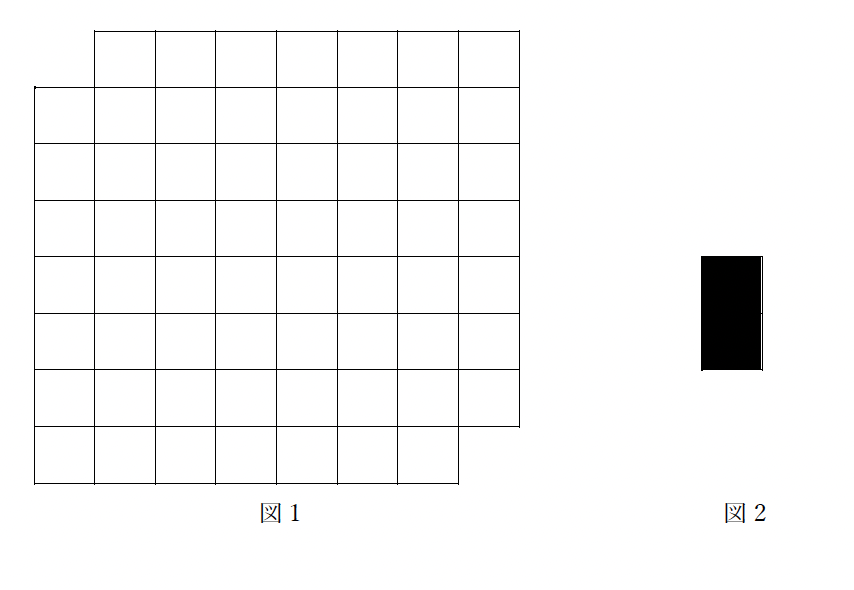
\includegraphics[width=60mm]{tile1.png}
\end{center}
\end{figure}

[答え]
下のように市松模様を描いたら, 赤色が32個, 白色が30個配置される.
そして2×1のタイルをどこに配置しても, 赤色と白色一つずつなくなっていく. 
よってもし2×1のタイルで埋め尽くされればそれは赤色と白色が同数でなければいけないが, この状況ではありえない.

\begin{figure}[htbp]
\begin{center}
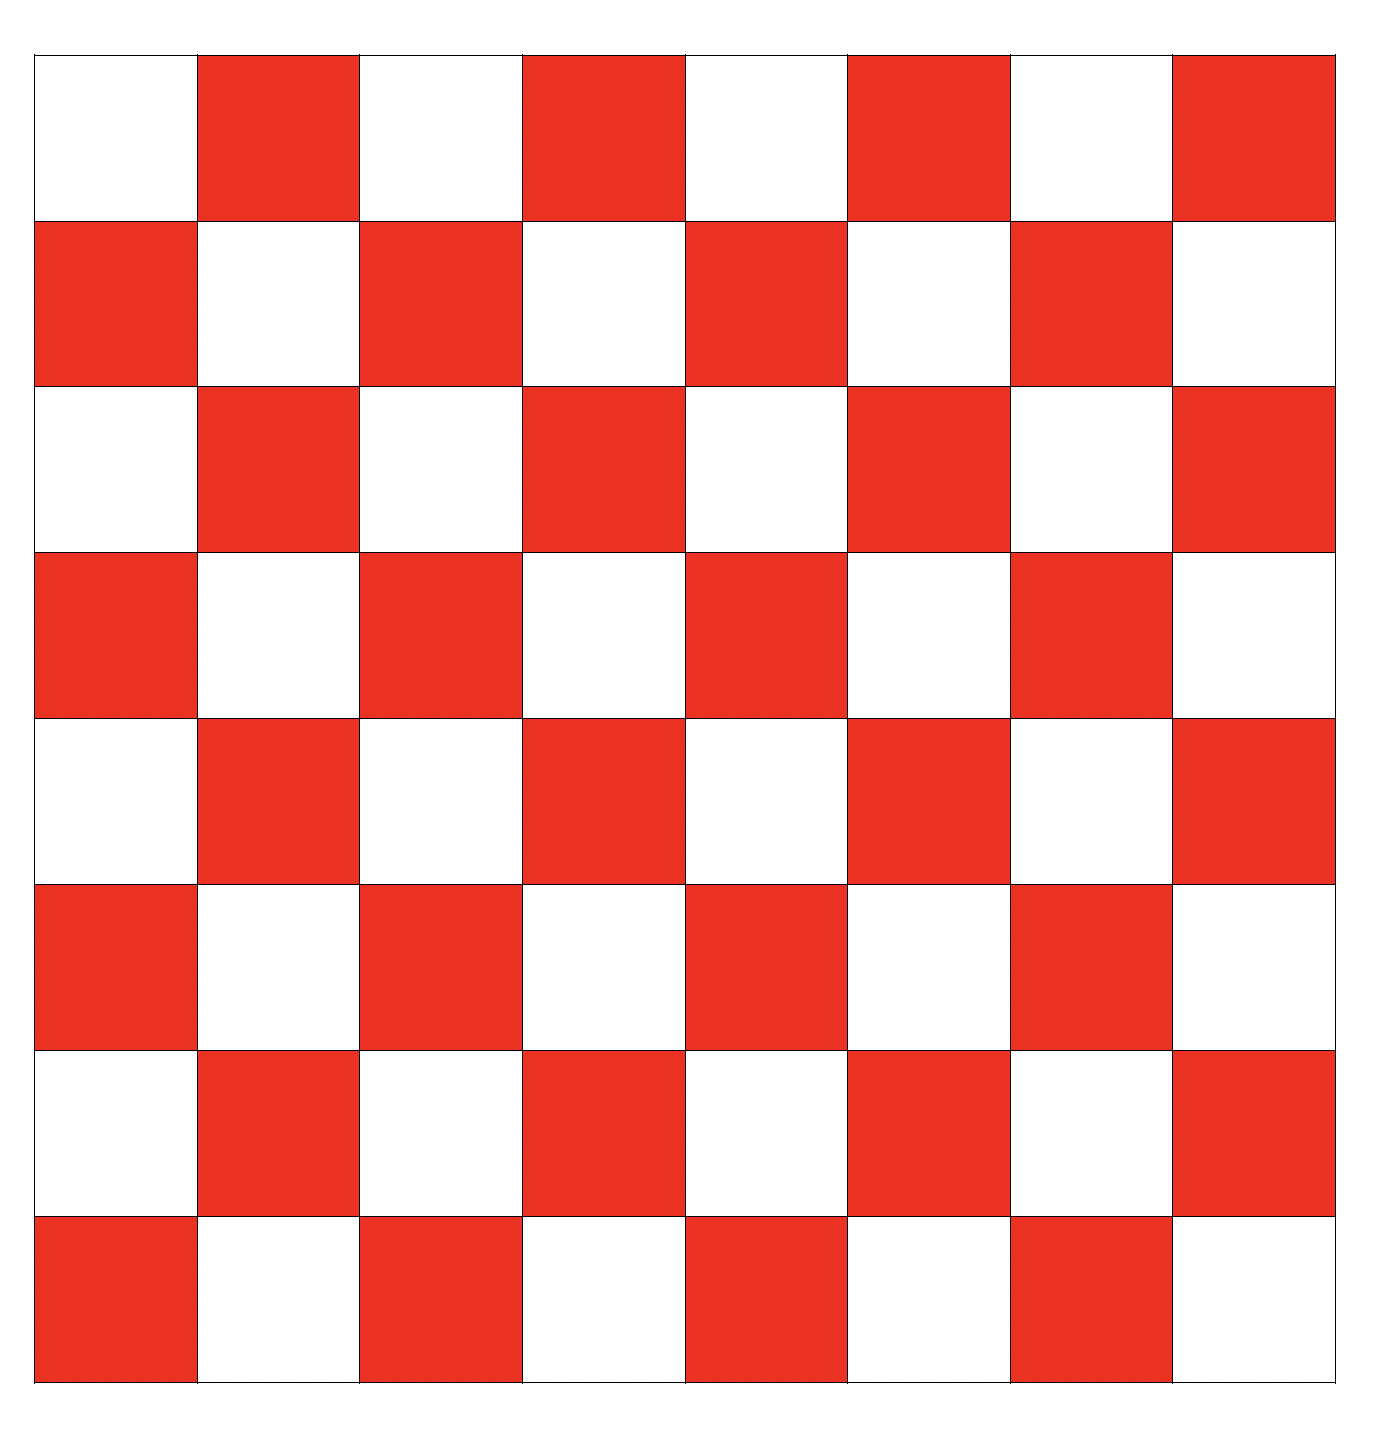
\includegraphics[width=80mm]{tile1_answer.png}
\end{center}
\end{figure}


\subsection{タイル2. }

\begin{tcolorbox}[mybox]
図1のような8×8のタイルの上に, 1×1タイルを好きなところにおく. 
このとき1×1タイルをどこにおいても, 図2のようなのタイルで埋め尽くすことができることを示せ.

ただし図2のようなタイルは重なり合ってはいけないしはみ出てはいけない.
\end{tcolorbox}

\begin{figure}[htbp]
\begin{center}
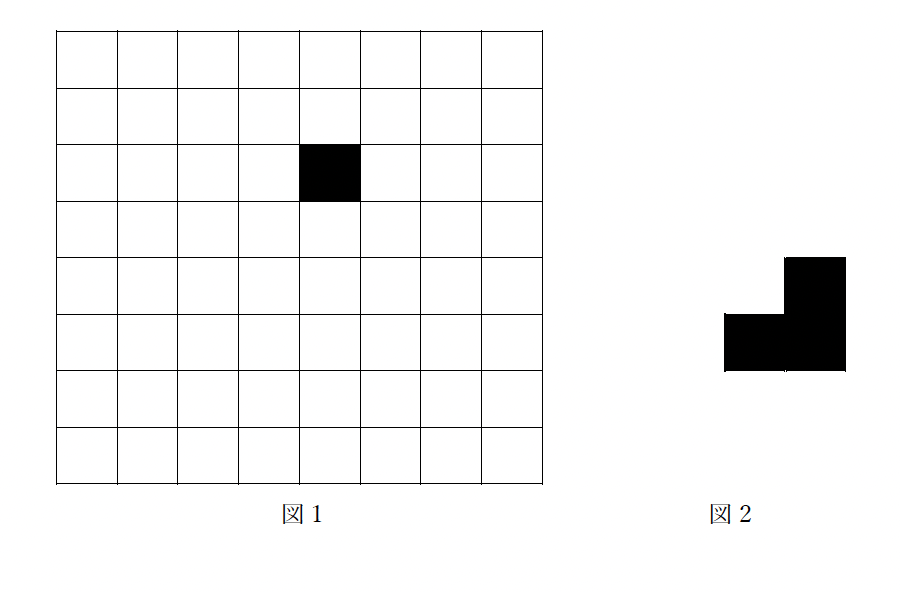
\includegraphics[width=80mm]{tile2.png}
\end{center}
\end{figure}

[答え]
実は$2^n$×$2^n$でもできる.

数学的帰納法を用いる. 
$n=2$の時は明らか. 

$n=k$の時にできると仮定して$n=k+1$の時にできることを示す. 
タイルを$2^k$×$2^k$タイルが4つになるように中心から4等分する.(下図のように赤緑青黄のように4等分する)
さて黄色の部分に1×1タイルを置いたとしよう. 
そして赤緑青に跨るようにタイルを置く
すると, 赤緑青黄の部分は$2^k$×$2^k$タイルから 1×1タイルが除かれたものなので, 帰納法の仮定より図2のようなのタイルで埋め尽くせる. 

以上よ数学的帰納法でいえた. $k=3$の場合が今回欲しい結果である. 

\begin{figure}[htbp]
\begin{center}
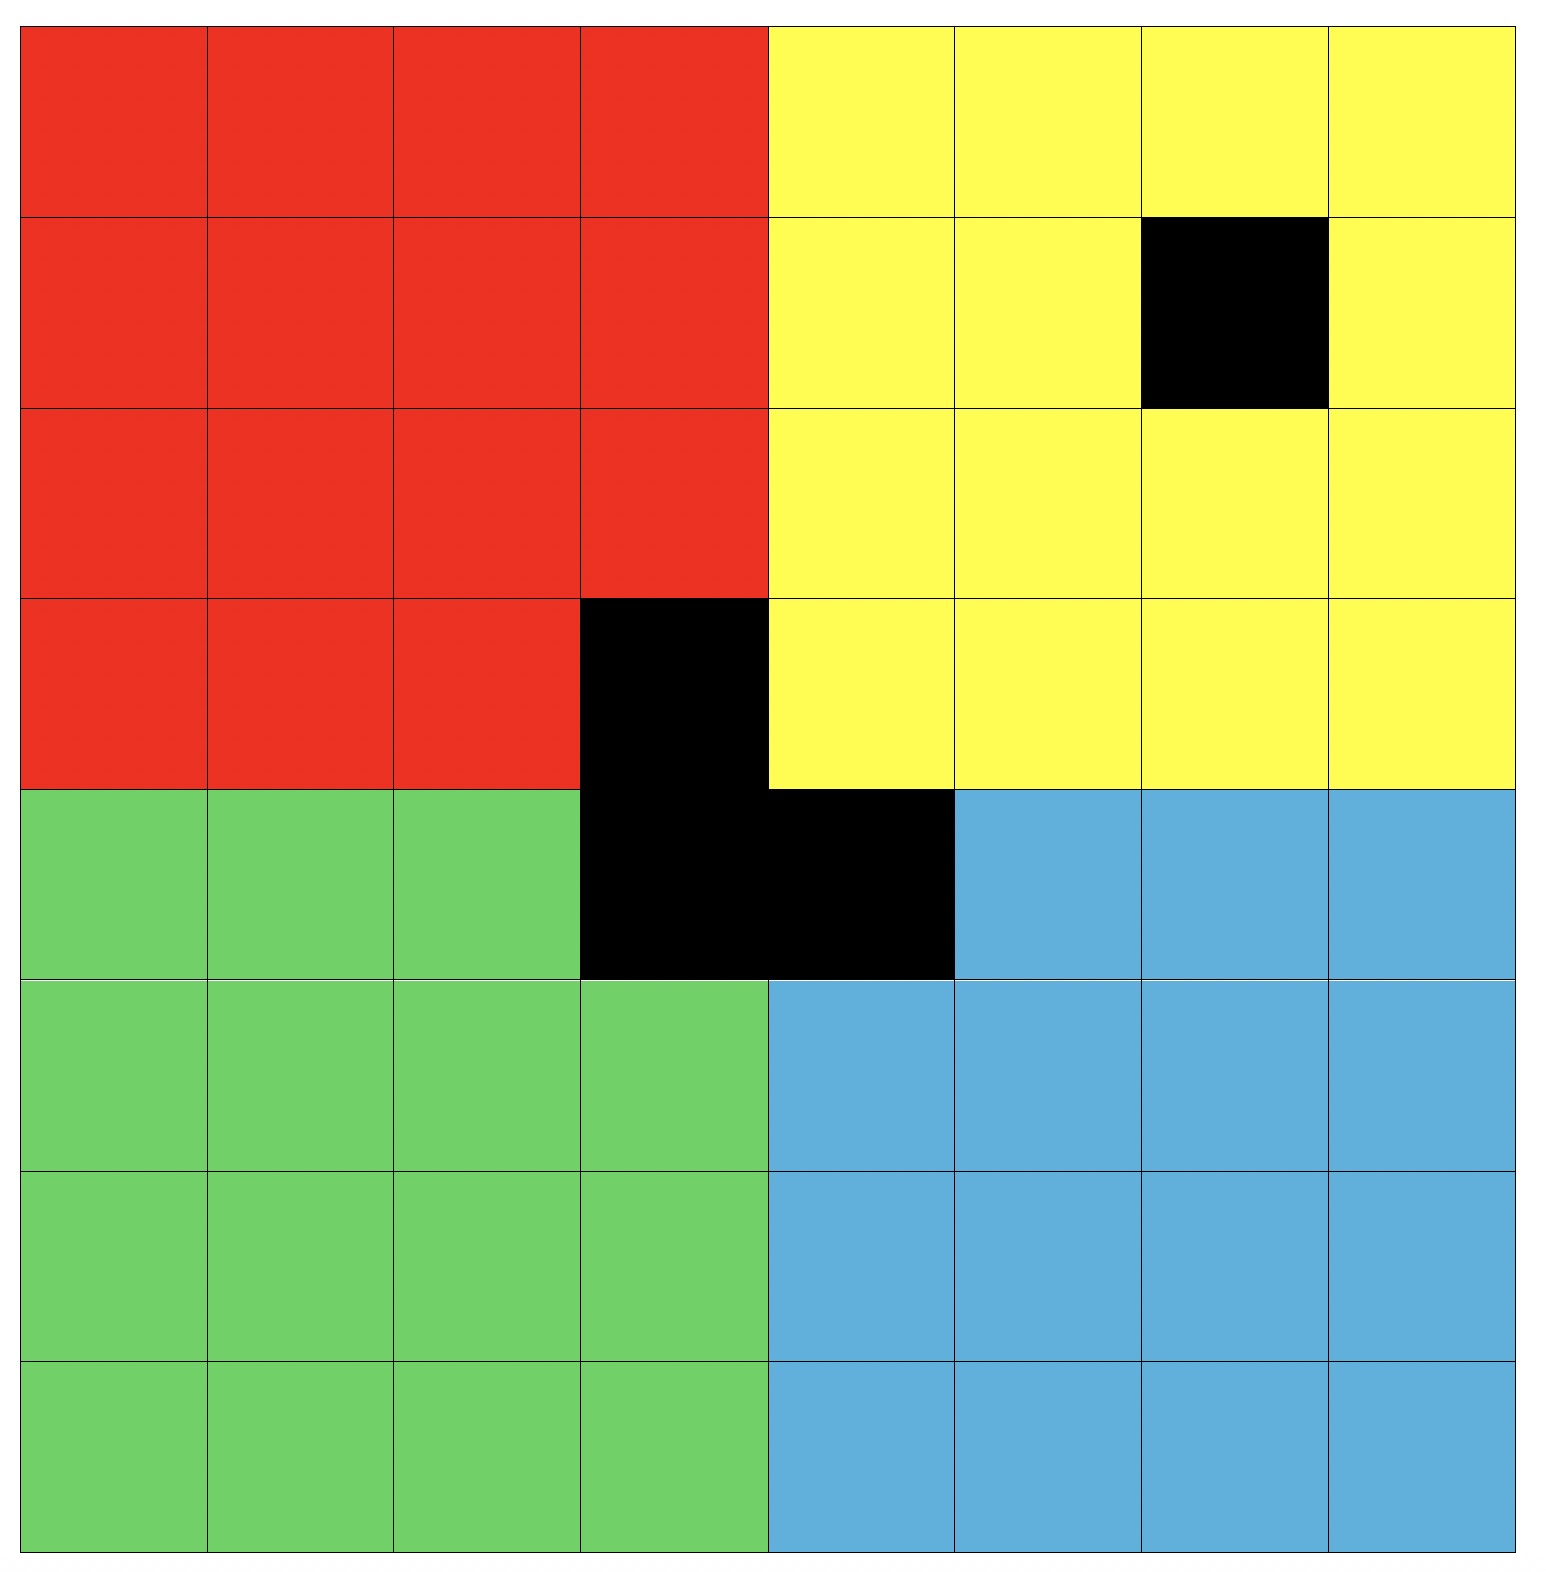
\includegraphics[width=60mm]{tile2_answer.png}
\end{center}
\end{figure}

\subsection{タイル3. }


\begin{tcolorbox}[mybox]
大きなタイルをたくさんの(有限個の)小さな長方形に分割した. 
その際全ての小さな長方形の縦の長さもしくは横の長さのどちらか(あるいは両方ともが)整数であった.

\vspace{5pt}
このとき, 大きな長方形の縦の長さもしくは横の長さのどちらか(あるいは両方とも)整数であることを示せ.

\end{tcolorbox}


\begin{figure}[htbp]
\begin{center}
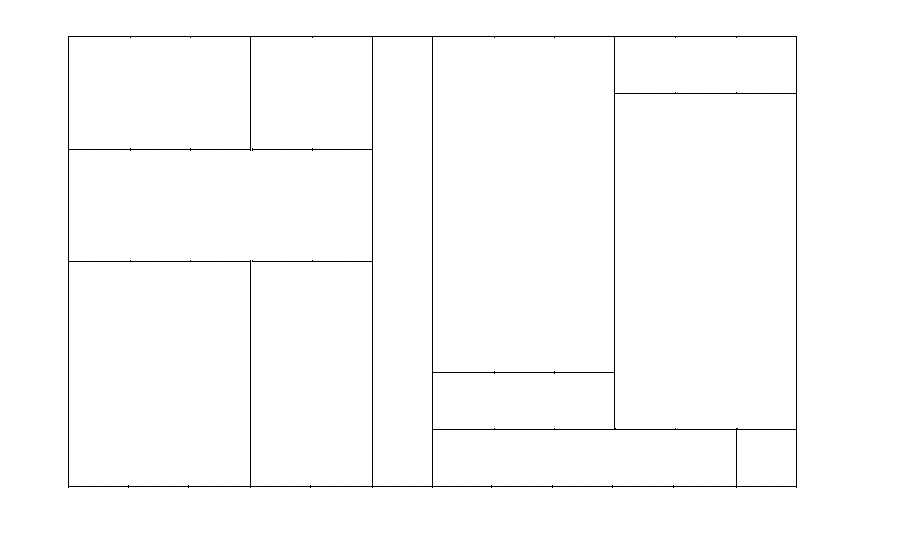
\includegraphics[width=80mm]{tile3.png}
\end{center}
\end{figure}

[答え]
一番簡単なのは下のように$\frac{1}{2} \times \frac{1}{2}$ずつ区切って, 市松模様を描く方法である. 
すると長方形の縦の長さもしくは横の長さのどちらか(あるいは両方ともが)整数ならば, 赤色と白色が同じ面積を持つことがわかる. 
逆に, 長方形の縦の長さと横の長さがどちらも整数でなければ, 赤色と白色が同じ面積を持たない. 

以上より, 小さな長方形の縦の長さもしくは横の長さのどちらか(あるいは両方ともが)整数なので, 赤色と白色が同じ面積を持つ. よって長方形の縦の長さと横の長さがどちらも整数でないことはありえない. 

\begin{figure}[htbp]
\begin{center}
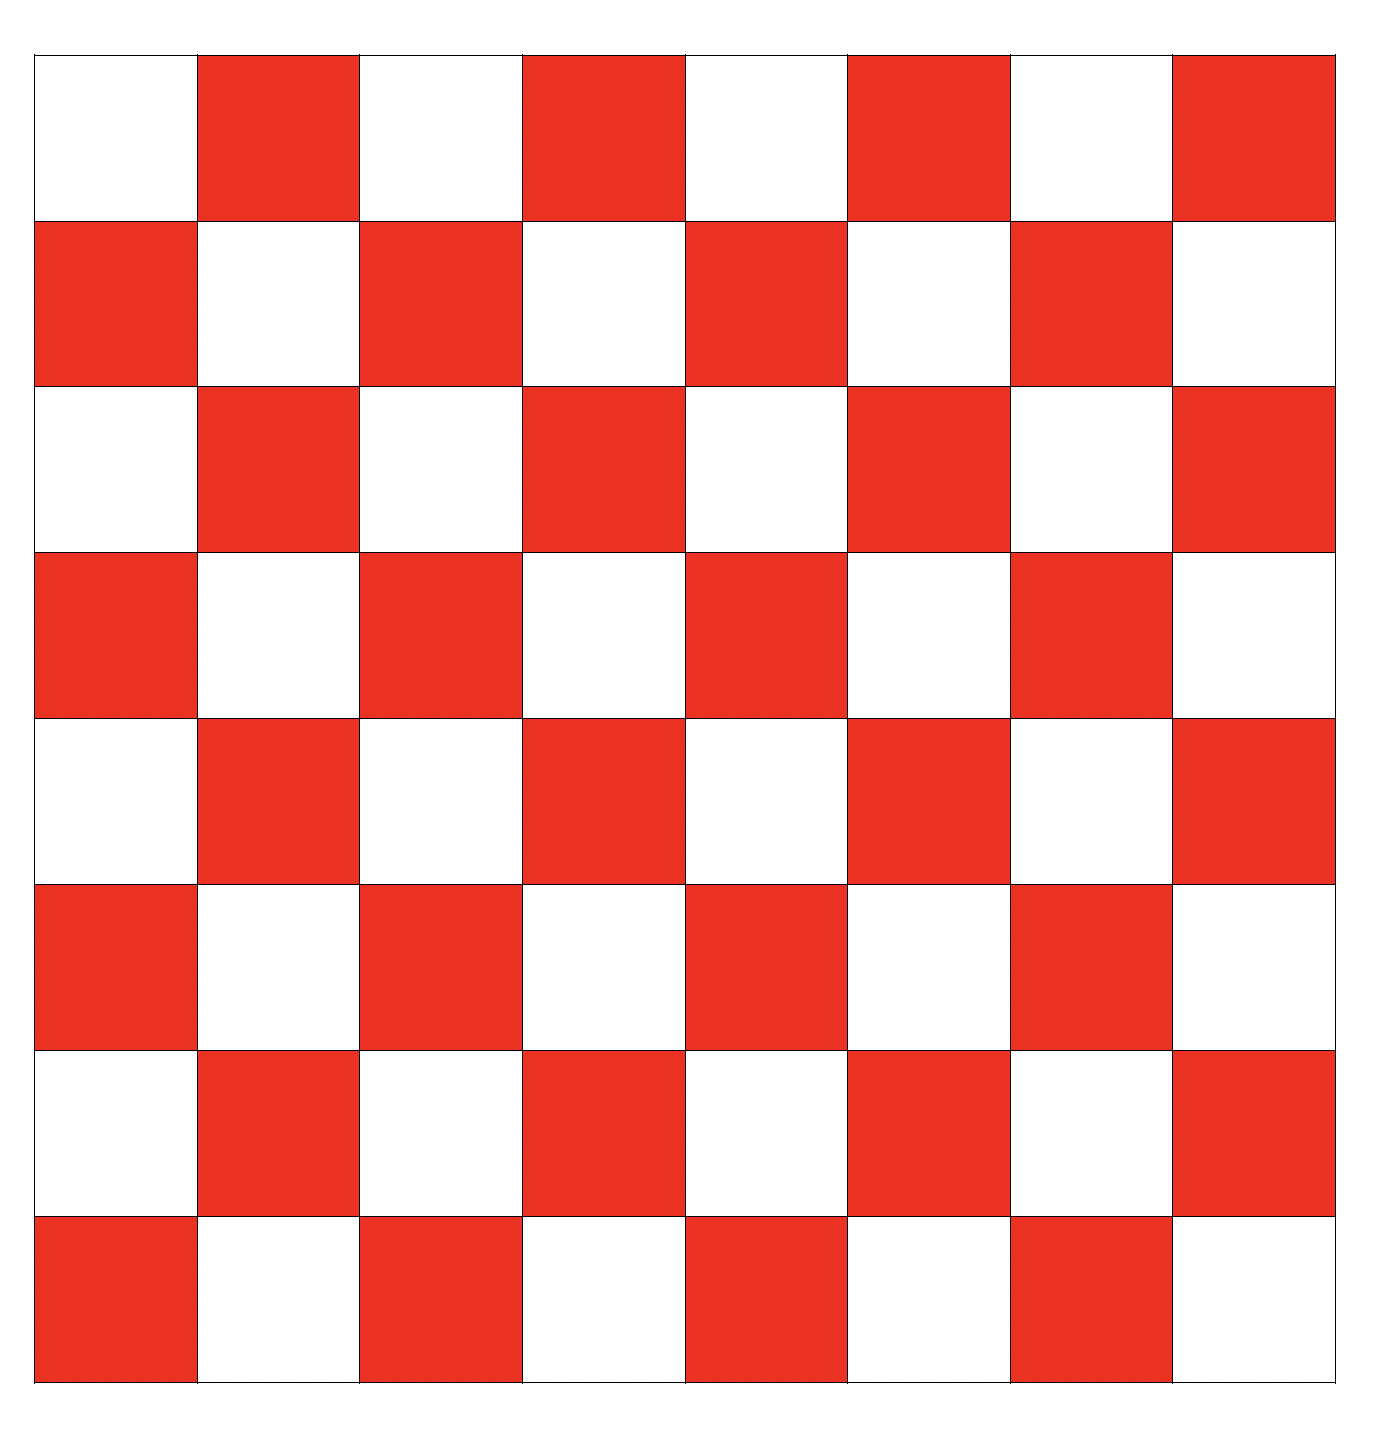
\includegraphics[width=60mm]{tile1_answer.png}
\end{center}
\end{figure}


\subsection{Kontsevichのパズル}
\begin{tcolorbox}[mybox]
図1のようにタイルが無限に並んでいて, 左下のみ黒で他は白であるものを考える.
次の操作を何回やっても, 図2の赤色の部分に黒のタイルがあることを示せ. 

\vspace{5pt}
[操作] 図1のように上も右も白であるような黒のタイルを選び, それを白タイルに変えて, その上も右も黒のタイルに変える.
\end{tcolorbox}
\begin{figure}[htbp]
\begin{center}
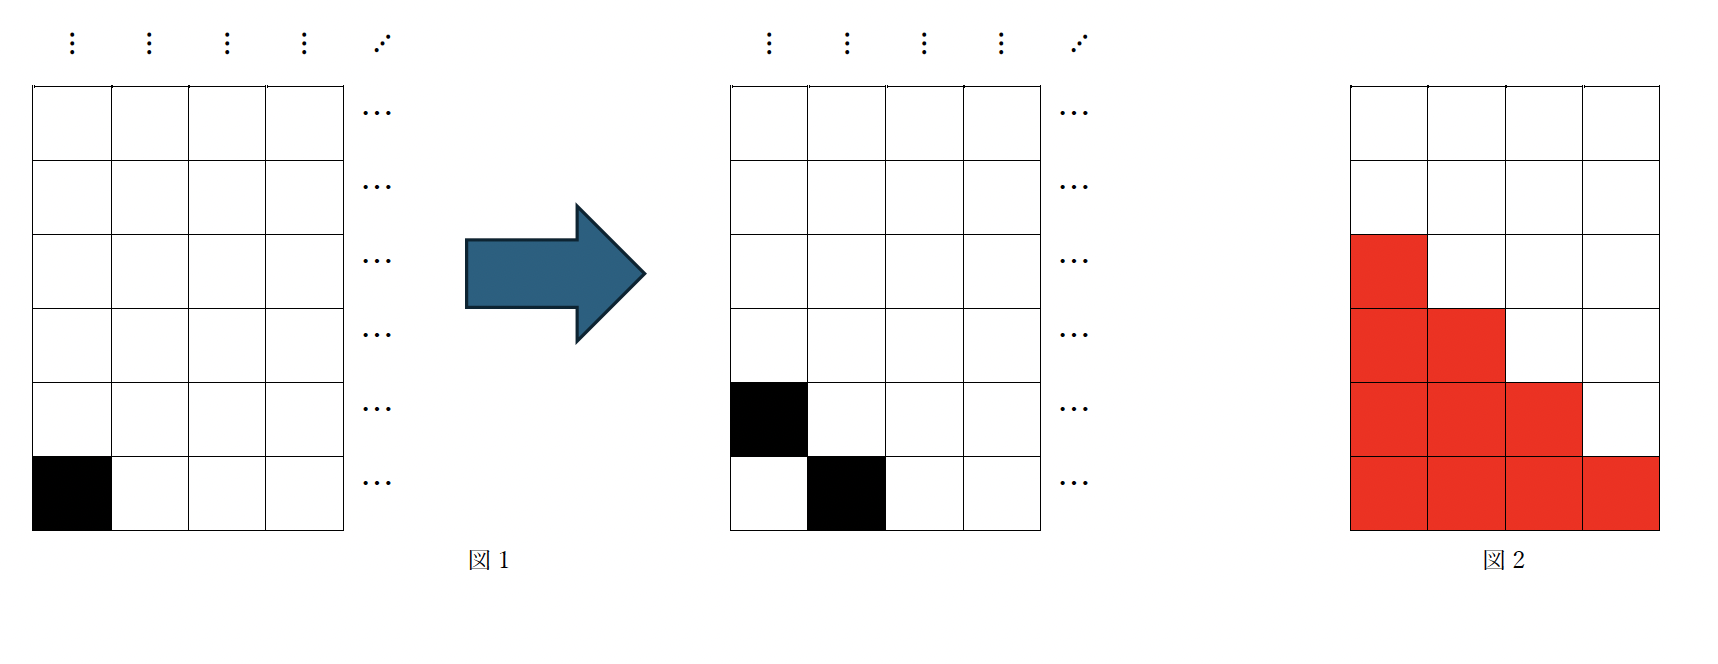
\includegraphics[width=100mm]{kont.png}
\end{center}
\end{figure}

[答え]
下図のように数を書いていく. 
(数学的にいうと, $(i,j)$成分のところに$\frac{1}{2^{i+j -2}}$を書く)
すると黒色のタイルが乗っている部分に書かれた数を全てたすと, 必ず1になる.
(つまり操作によってこの量は不変である)

あとは背理法. もし図2の赤色の部分に黒のタイルがなければ, 
その時の黒色の部分の総和$S$は, 図2の赤色の部分以外の和以下なので, 
$$
S \le \frac{5}{16}+\frac{6}{32}+ \frac{7}{64}+  \cdots = \frac{3}{4}
$$
しかし黒色の部分の総和は$1$でないといけないので矛盾. 

\begin{figure}[htbp]
\begin{center}
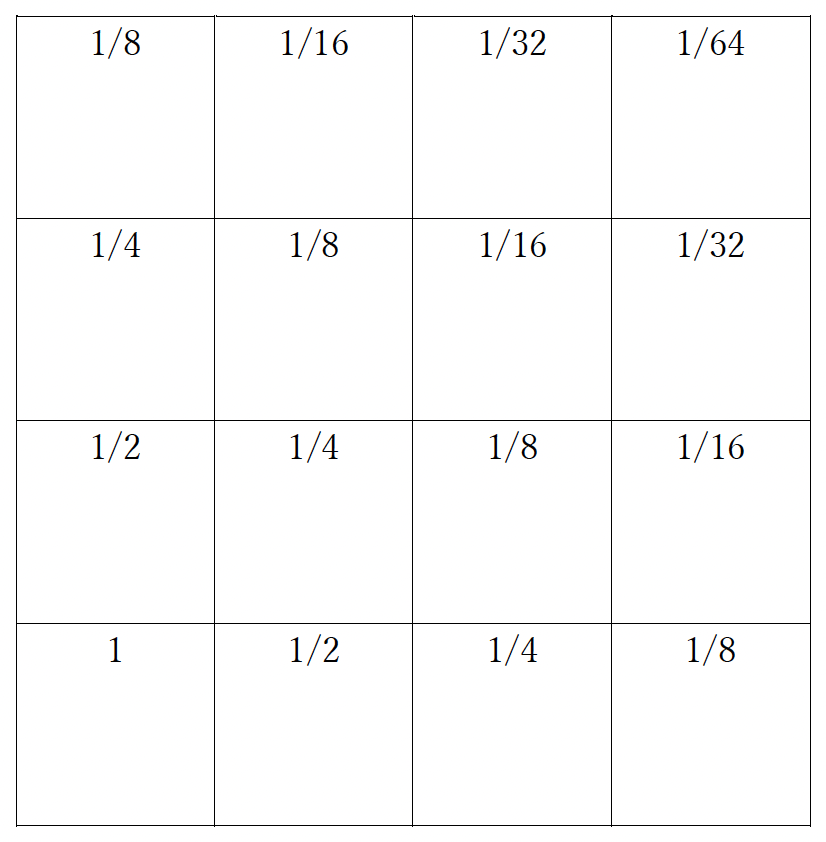
\includegraphics[width=60mm]{kont_answer.png}
\end{center}
\end{figure}


\subsection{ドブル}

\begin{tcolorbox}[mybox]
7色(赤, 橙, 黄, 緑, 青, 藍, 紫) のペンと7枚のカードある. 次のルールを考える.
\begin{enumerate}
    \setlength{\parskip}{0cm} 
  \setlength{\itemsep}{0cm} 
\item どのカードにも相異なる3 色の$\bullet$印がある.
\item どの2 枚のカードを取っても, 1 つだけ共通する色の$\bullet$印がある.
\end{enumerate}
上のルール2 つを満たすように色ペンを使ってカードに$\bullet$印を書くことはできるだろうか?
\end{tcolorbox}

[答え(簡単版)]
まあ7個なので下の図が答えになる.
\begin{figure}[htbp]
\begin{center}
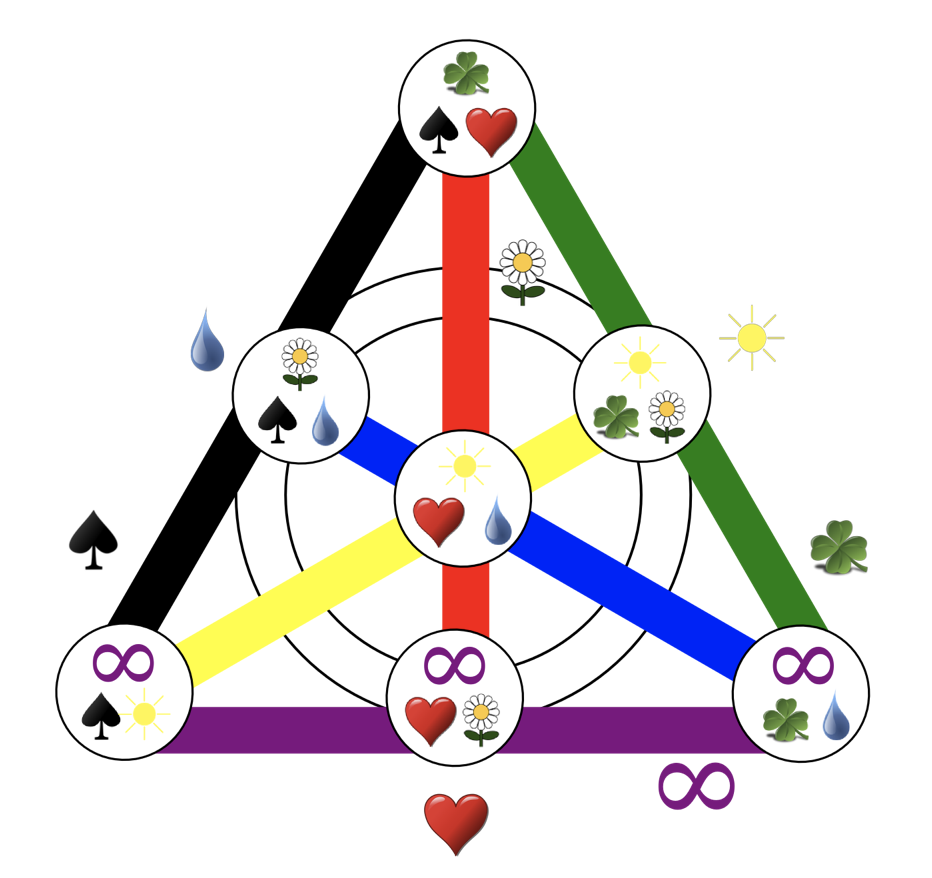
\includegraphics[width=50mm]{dobble_answer.png}
\end{center}
\end{figure}
なお\url{https://math.stackexchange.com/questions/36798/what-is-the-math-behind-the-game-spot-it}の画像を拝借した.

この図が言っていることは以下の通り.
\begin{itemize}
\item 7点にカードを対応させる.
\item 直線や円に色(赤, 橙, 黄, 緑, 青, 藍, 紫)を対応させる.
\end{itemize}

[答え(難しい版)]
$p$を素数として, その2次元射影空間$X=F_p\mathbb{P}^{2}$を考える. 
$X$の点の個数は$\frac{p^3 - 1}{p-1}=p^2 + p^1 + 1$である.
そこで次を考える.
\begin{itemize}
\item $X$の点にカードを対応させる.
\item $X$の直線に色を対応させる.
\end{itemize}

すると次がわかる.
\begin{itemize}
\item 相異なる直線3つを通る点はただ一つに定まる. 
これは"どのカードにも相異なる3 色の$\bullet$印がある"に対応する. 
\item 二つの異なる点を結ぶ直線はただ一つに定まる. 
これは"どの2 枚のカードを取っても, 1 つだけ共通する色の$\bullet$印がある"に対応する. 
\end{itemize}
今$p=3$の場合は$2^2 + 2^1 + 1=7$よりできる. 

なお$p=7$の時は$7^2 + 7^1 + 1=57$である. 
ポケモンのドブルに出てくるポケモンの数は57匹である. (ちなみにカード数はなぜか55枚である. 57枚でもできる.) 

\subsection{11111.....}

\begin{tcolorbox}[mybox]
$p$を2や5でない素数とする. 
$11111\cdots 111$という1が何個か並んだ形の$p$の倍数が存在することを示せ.
\end{tcolorbox}

[答え]
$a_n$を$1$が$n$個並んだ数を$p$で割ったあまりとする. 
すると$a_1, a_2, \ldots, a_{p}, a_{p+1} \in \{0, \ldots, p-1\}$であるので, 鳩の巣論法より, 
$a_i =a_j$となる$i<j$が存在する(もし全て異なっていたら$\{0, \ldots, p-1\}$の中に$p+1$この数が含まれてしまう!)

そこで
$$\underbrace{11111\cdots 111}_{\text{$j$個}} - 
\underbrace{11111\cdots 111}_{\text{$i$個}} $$
  を考える. 
  するとこれを$p$であったあまりは$a_j - a_i$に等しく, それは0となる. 
 よって
$$
\underbrace{11111\cdots 111}_{\text{$j$個}} - 
\underbrace{11111\cdots 111}_{\text{$i$個}} 
=
\underbrace{11111\cdots 111}_{\text{$j-i$個}} \times 10^{i}$$
を$p$であったあまりも0となる. 

$p$を2や5でない素数なので
$10^{i}$は$p$で割り切れない.  よって$\underbrace{11111\cdots 111}_{\text{$j-i$個}}$が$p$で割り切れる. 


\subsection{2010年大阪大学理系第3問}

\begin{tcolorbox}[mybox]
$l,m,n$を3以上の整数とする. 等式
$$
\left( \frac{n}{m} - \frac{n}{2} + 1 \right)l = 2
$$
を満たす$l,m,n$の組を全て求めよ. 
\end{tcolorbox}

[解説]
おそらく有名な問題なので解答は割愛する. 
答えは
$$
(l,m,n)
=(4,3,3), (6,3,4), (8,4,3), (12,3,5), (20,5,3)
$$
である. 
要は正多面体が5個しかないことの整数的な解釈となる. 
まあこの問題の答えや正多面体の話はネットにいっぱい乗っているので, 別の話をする. 

この問題の要はオイラーの多面体定理である. 
ざっくりゆうと
\begin{tcolorbox}[mybox]
球と同相な多面体の面の数$F$, 辺の数$E$, 頂点の数$V$とすると
$$
F-E +V=2
$$
が成り立つ
\end{tcolorbox}


数学科の展示に正多胞体がある. この場合には
$$
\text{胞(立体)の数}-\text{面の数}+\text{辺の数}-\text{頂点の数}=0
$$
となる. 
この右辺に現れる$2$や$0$は実は$n$次元球面$S^n$のオイラー数である.
$$
\text{$S^2$のオイラー数}=2 
\quad
\text{$S^3$のオイラー数}=0
$$
である.
 実は一般に$m$を整数として, $\text{$S^{2m}$のオイラー数}=2$, $\text{$S^{2m+1}$のオイラー数}=0$である.
 なので, 5次元に行った場合でも
$$
\text{5次元立体の数}-\text{4次元立体の数}+\text{3次元立体の数}-\text{面の数}+\text{辺の数}-\text{頂点の数}=0
$$
となる. 

ちなみにこの式だけで正多胞体を分類することはできない. 
4次元の正多胞体を
$$
\text{胞(立体)の数}-\text{面の数}+\text{辺の数}-\text{頂点の数}=0
$$
を用いて分類すると11種類の可能性が出てくる. 
しかしあり得るのは6種類である. なので残りの5種類は幾何学的な条件(シュレフリー条件)を満たさないので弾かれる. 



\subsection{コイン 1}
\begin{tcolorbox}[mybox]
テーブル上に10個の硬貨が一列に並んでいる. 
その硬貨の額は1円か5円か10円である. 

あなたと私の二人で次のルールの下, 以下のゲームを行う.
\begin{itemize}
\item 列のうち左端か右端の硬貨を取る. その後次の人に手番をわたす.
\item とった硬貨の総額が多い方が勝ち. 同じであれば引き分け. 
\end{itemize}

ゲームに"負けたくない"あなたなら先手・後手どちらを選べば良いだろうか?
またその際どのような戦略を取れば良いだろうか?
\end{tcolorbox}
\begin{figure}[htbp]
\begin{center}
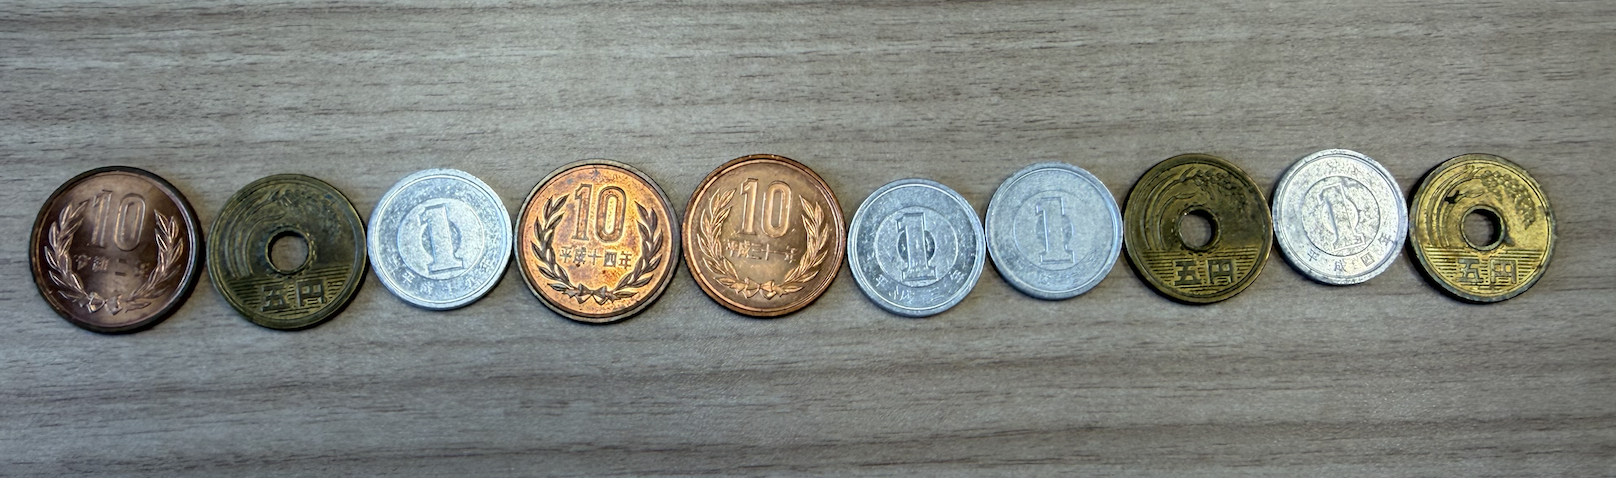
\includegraphics[width=80mm]{coin1.png}
\end{center}
\end{figure}

[答え]
やはり市松模様を考える. するとこのルールの元では一回赤色の上のコインをとると, ゲームが終わるまで赤色のコインを取り続けることになる. 

なのでゲームに"負けたくない"あなたは先手を選び, 赤色の上のコインの総額と白色の上のコインの総額のうち大きい方を選べば, 負けることはない(ただし引き分けはありうる)
\begin{figure}[htbp]
\begin{center}
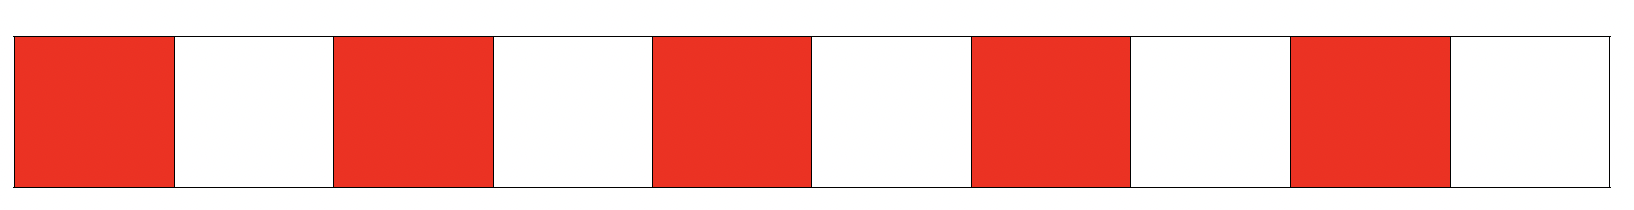
\includegraphics[width=80mm]{coin1_answer.png}
\end{center}
\end{figure}


\subsection{コイン 2}

\begin{tcolorbox}[mybox]
テーブル上に25個の1円玉がある.
あなたと私の二人で次のルールの下, 以下のゲームを行う.

\begin{itemize}
\item テーブルの上の1円玉から, 1枚か2枚か3枚のコインを取る. その後次の人に手番をわたす.
\item 最後の1円玉を取った人が負け.
\end{itemize}

ゲームに"負けたくない"あなたなら先手・後手どちらを選べば良いだろうか?
またその際どのような戦略を取れば良いだろうか?
\end{tcolorbox}

\begin{figure}[htbp]
\begin{center}
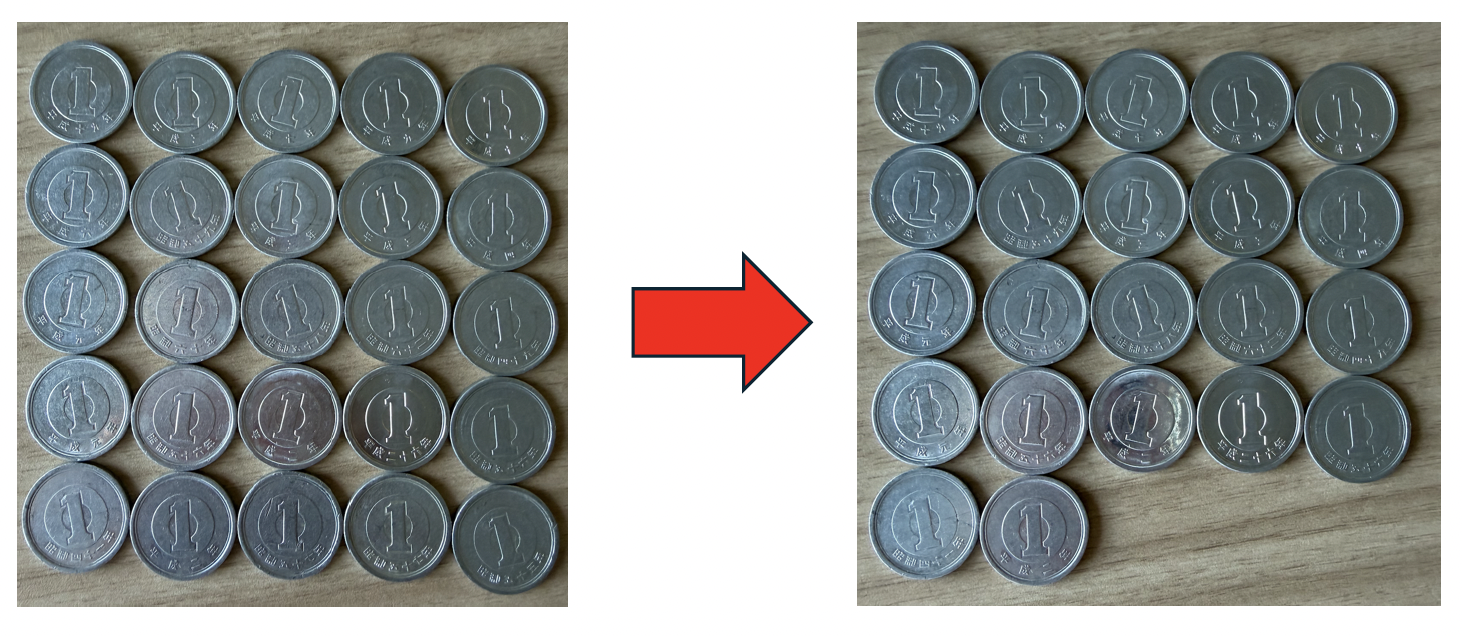
\includegraphics[width=80mm]{coin2.png}
\end{center}
\end{figure}

[答え]
こういう問題は1円玉の枚数が少ない状態から始めるのが吉である.
\begin{itemize}
\item 1枚の時. この場合は先手の負けである.
\item 2枚の時. この場合は先手には次の2つの手がある. 
\begin{enumerate}
\item 1枚とる. この時後手は"1枚の状況になる(負けの状況)"になるので, 先手の勝ち(後手の負け)
\item 2枚とる. 負けが確定.
\end{enumerate}
よってこの場合は先手の勝ちで, 初手で1枚取れば良い.
\item 3枚の時. 先手には次の3つの手がある.
\begin{enumerate}
\item 1枚とる. この時後手は"2枚の状況になる(勝ちの状況)"になるので, 先手の負け(後手の勝ち)
\item 2枚とる. この時後手は"1枚の状況になる(負けの状況)"になるので, 先手の勝ち(後手の負け)
\item 3枚とる. 負けが確定.
\end{enumerate}
よってこの場合は先手の勝ちで, 初手で1枚取れば良い.
\item  4枚の時. (省略すると)先手の勝ち
\item  5枚の時. (省略すると)先手の勝ち 先手には次の3つの手がある.
\begin{enumerate}
\item 1枚とる. この時後手は"4枚の状況になる(勝ちの状況)"になるので, 先手の負け(後手の勝ち)
\item 2枚とる.  この時後手は"3枚の状況になる(勝ちの状況)"になるので, 先手の負け(後手の勝ち)
\item 3枚とる.  この時後手は"2枚の状況になる(勝ちの状況)"になるので, 先手の負け(後手の勝ち)
\end{enumerate}
よってこの場合は先手の負けである.
\end{itemize}

よってコインの枚数を$n$として, $g(n)$を$W$(先手の勝ち)か$L$(先手の負け)とした場合
\begin{itemize}
\item $g(n-1)=L$か$g(n-2)=L$か$g(n-3)=L$ならば$g(n)=W$とする. 
これは先手が$n$枚から$1\sim3$枚取れば, 後手が必ず負けるような枚数になっているから.
\item $g(n-1)=g(n-2)=g(n-3)=W$ならば$g(n)=L$
これは先手が$n$枚から$1\sim3$枚をどう取っても, 後手が必ず勝つ枚数になっているから.
\end{itemize}
というように$g(n)$を定める.

下の図は$g(n)=L$を赤色にした図である
\begin{figure}[htbp]
\begin{center}
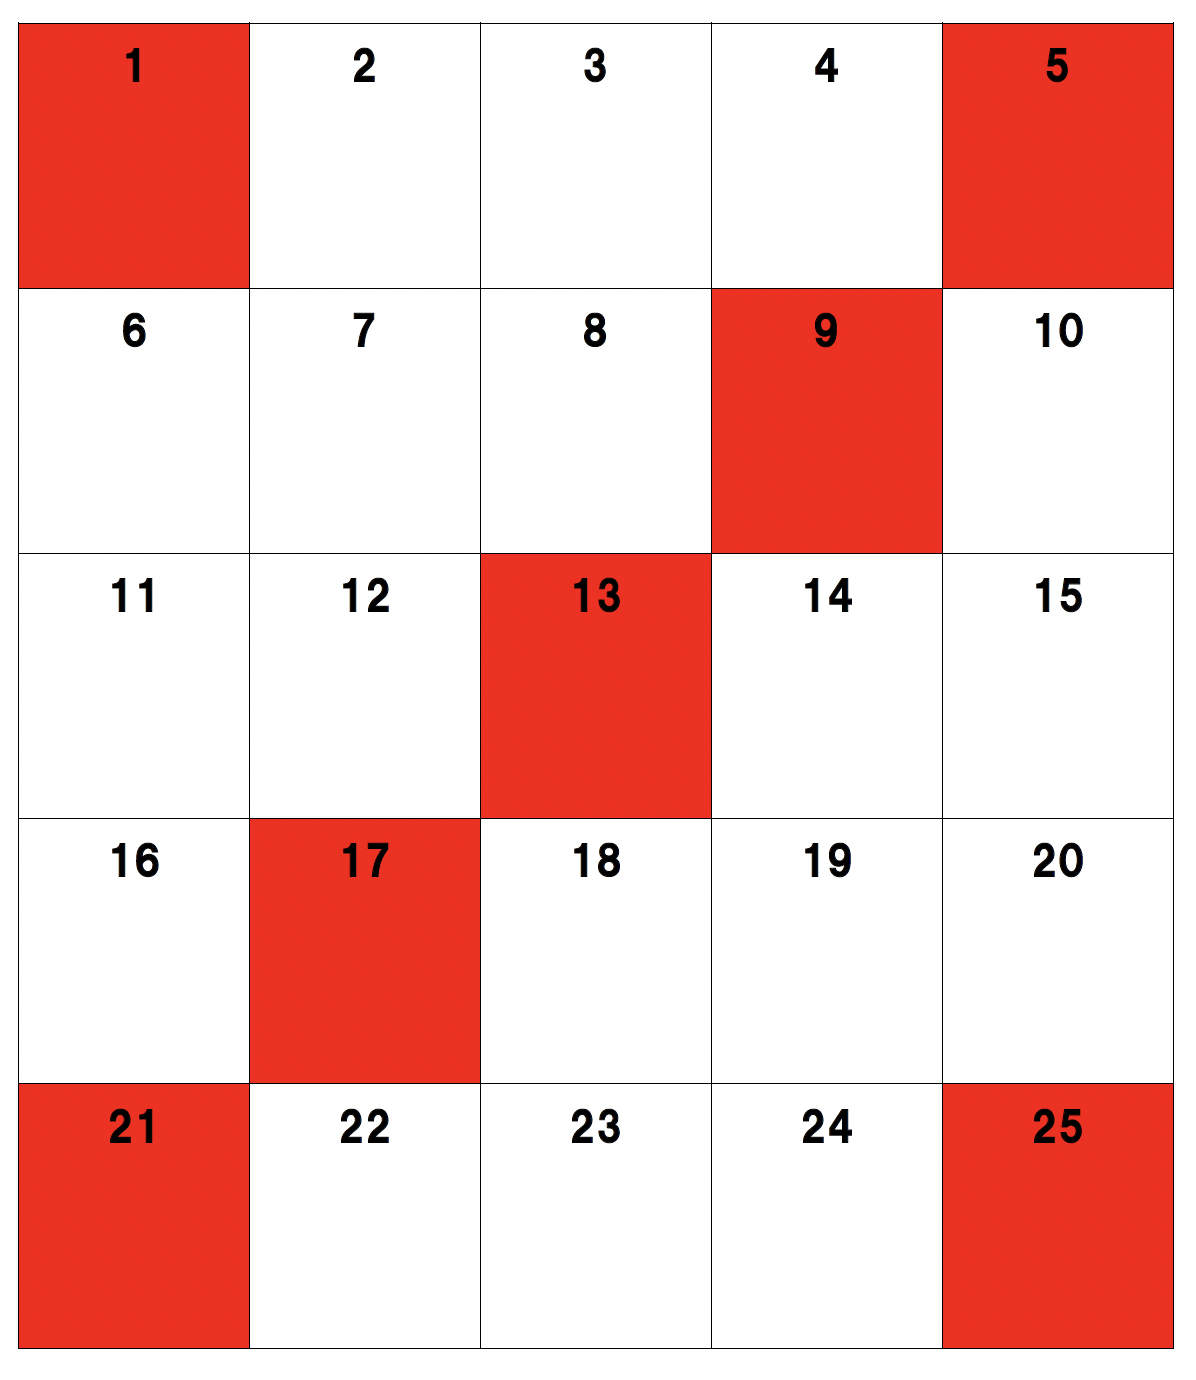
\includegraphics[width=50mm]{coin2_answer.png}
\end{center}
\end{figure}

この図を見ると$g(25)=L$より先手は負ける(後手必勝)
後手の動き方は"相手が$g(l)=L$"となるような$l$枚の状況になるように石を取る. 
もっと平たくいうと必勝法は
$$
\text{先手が赤色のコインを必ず取るように, コインをとっていく}
$$
である.つまり赤色の直前のコインまで取れば良い. 


\subsection{コイン 2'}
\begin{tcolorbox}[mybox]
テーブル上に25個の1円玉がある.
あなたと私の二人で次のルールの下, 以下のゲームを行う.

\begin{itemize}
\item テーブルの上の1円玉から, \underline{1枚か3枚か4枚}のコインを取る. その後次の人に手番をわたす.
\item 最後の1円玉を取った人が負け.
\end{itemize}


ゲームに"負けたくない"あなたなら先手・後手どちらを選べば良いだろうか?
またその際どのような戦略を取れば良いだろうか?
\end{tcolorbox}

[答え]

よってコインの枚数を$n$として, $g(n)$を$W$(先手の勝ち)か$L$(先手の負け)とした場合
\begin{itemize}
\item $g(n-1)=L$か$g(n-3)=L$か$g(n-4)=L$ならば$g(n)=W$とする. 
これは先手が$n$枚から$1, 3, 4$枚取れば, 後手が必ず負けるような枚数になっているから.
\item $g(n-1)=g(n-3)=g(n-4)=W$ならば$g(n)=L$
これは先手が$n$枚から$1, 3, 4$枚をどう取っても, 後手が必ず勝つ枚数になっているから.
\end{itemize}
というように$g(n)$を定める.

下の図は$g(n)=L$を赤色にした図である
\begin{figure}[htbp]
\begin{center}
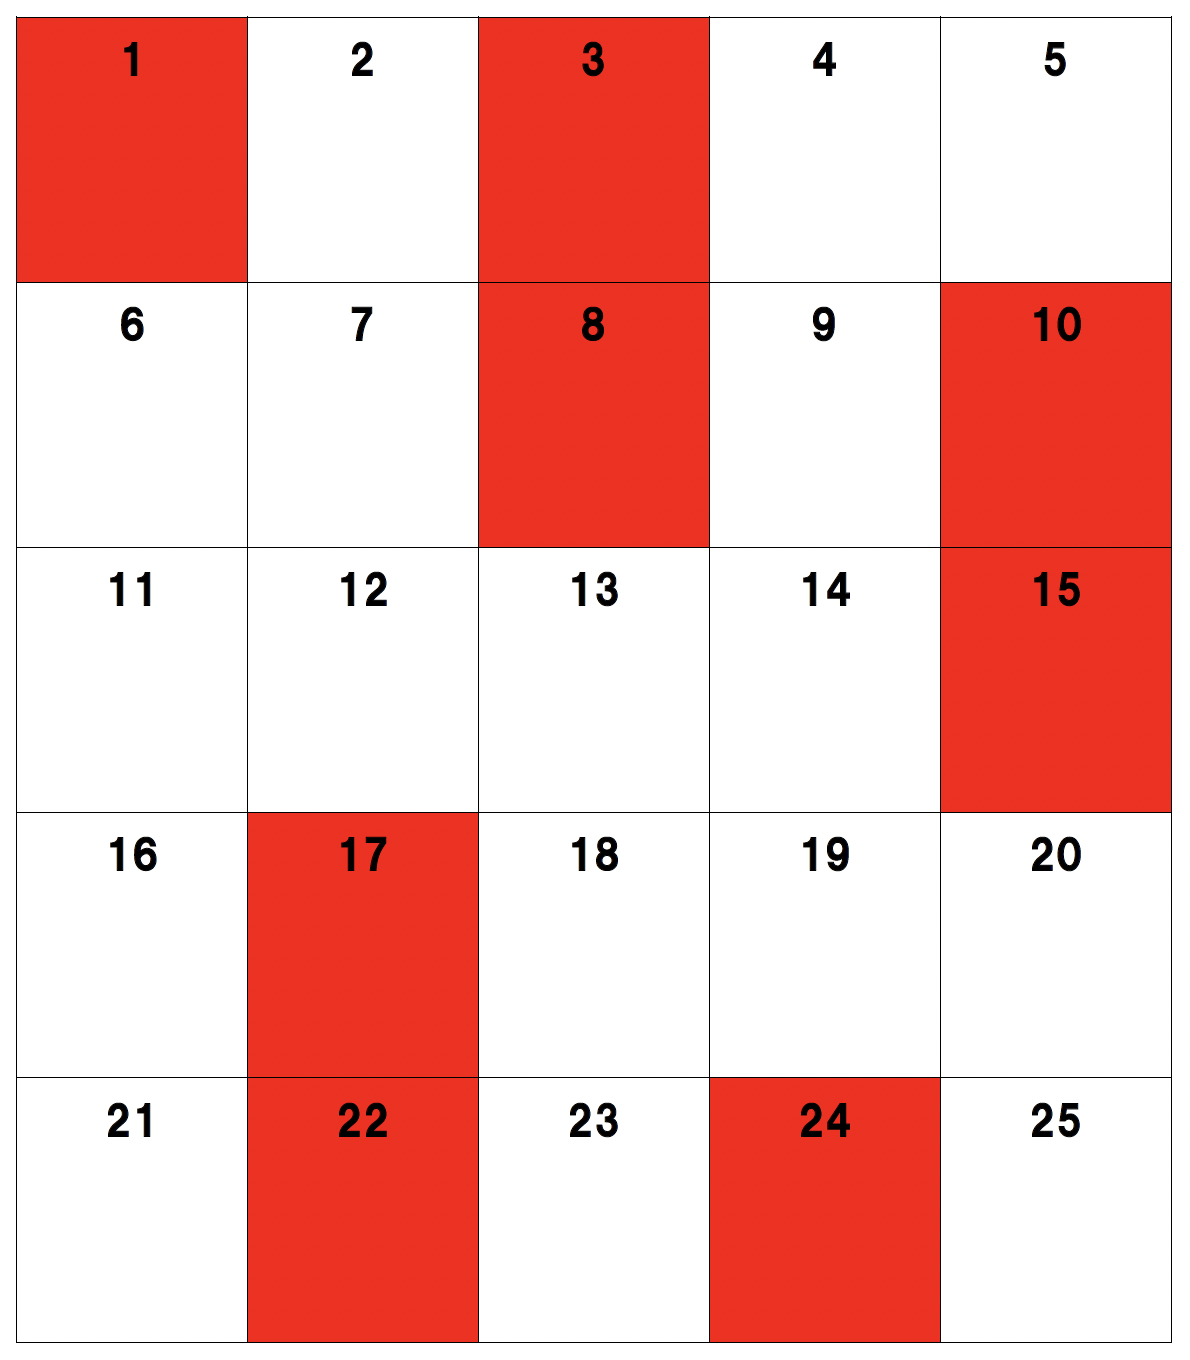
\includegraphics[width=50mm]{coin22_answer.png}
\end{center}
\end{figure}

この図を見ると$g(25)=W$より先手は勝つ
後手の動き方は"相手が$g(l)=L$"となるような$l$枚の状況になるように石を取る. 
もっと平たくいうと必勝法は
$$
\text{後手が赤色のコインを必ず取るように, コインをとっていく}
$$
である.つまり赤色の直前のコインまで取れば良い. 


\subsection{コイン 3}
\begin{tcolorbox}[mybox]
1円玉が裏向きに$5 \times 5$の正方形に並んでいる.
次の操作を考える. 
\begin{itemize}
\item 縦か横に連続する3枚の1円玉を同時にひっくり返す.
\end{itemize}

 この操作を何回かして全ての1円玉を表向きにできるか?
 \end{tcolorbox}
 
 \begin{figure}[htbp]
\begin{center}
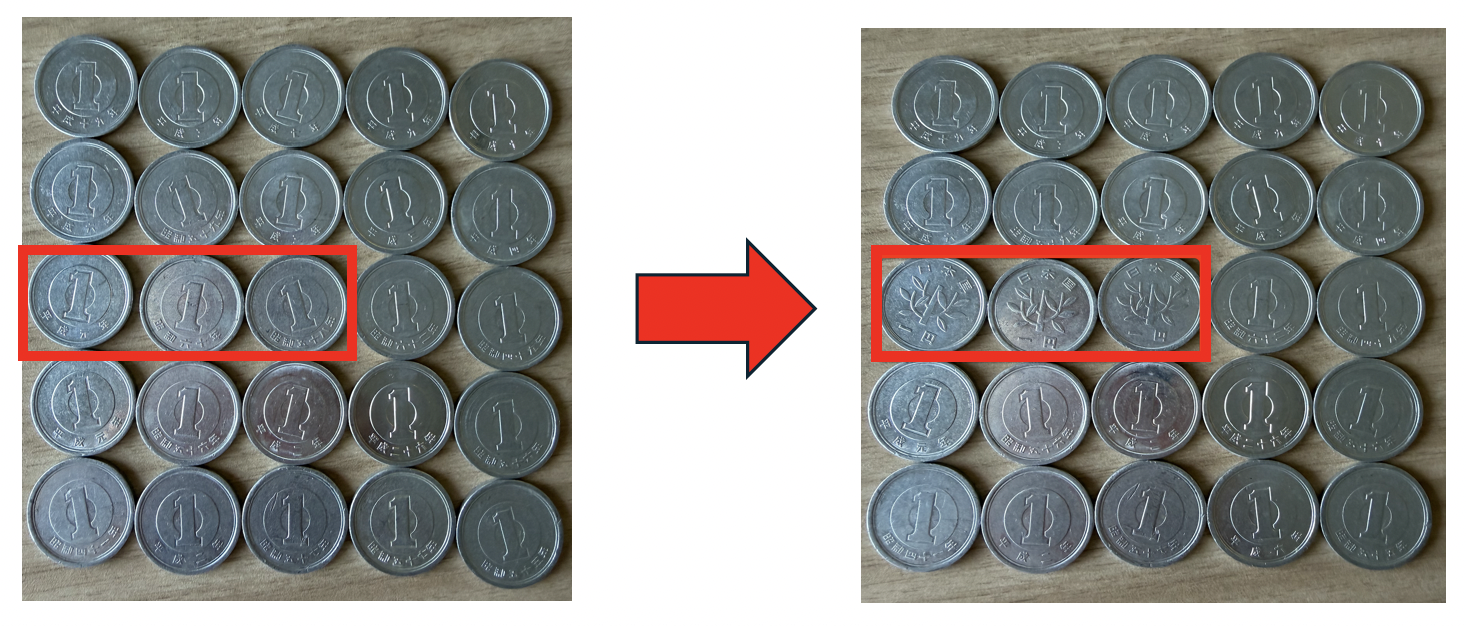
\includegraphics[width=80mm]{coin3.png}
\end{center}
\end{figure}

[答え]
できない. 下のように赤青白で塗る.
赤は9枚, 青白8枚である. 

もしできたとすると, 赤の上のコインをひっくり返すのには奇数回かかることになる. 
一方で青・白の上のコインをひっくり返すのには偶数回かかることになる. 

しかしこの操作では赤青白のコインが一斉にひっくり返るので, コインをひっくり返す回数の偶奇は赤・青・白で一致しないといけないので, 矛盾. 
 \begin{figure}[htbp]
\begin{center}
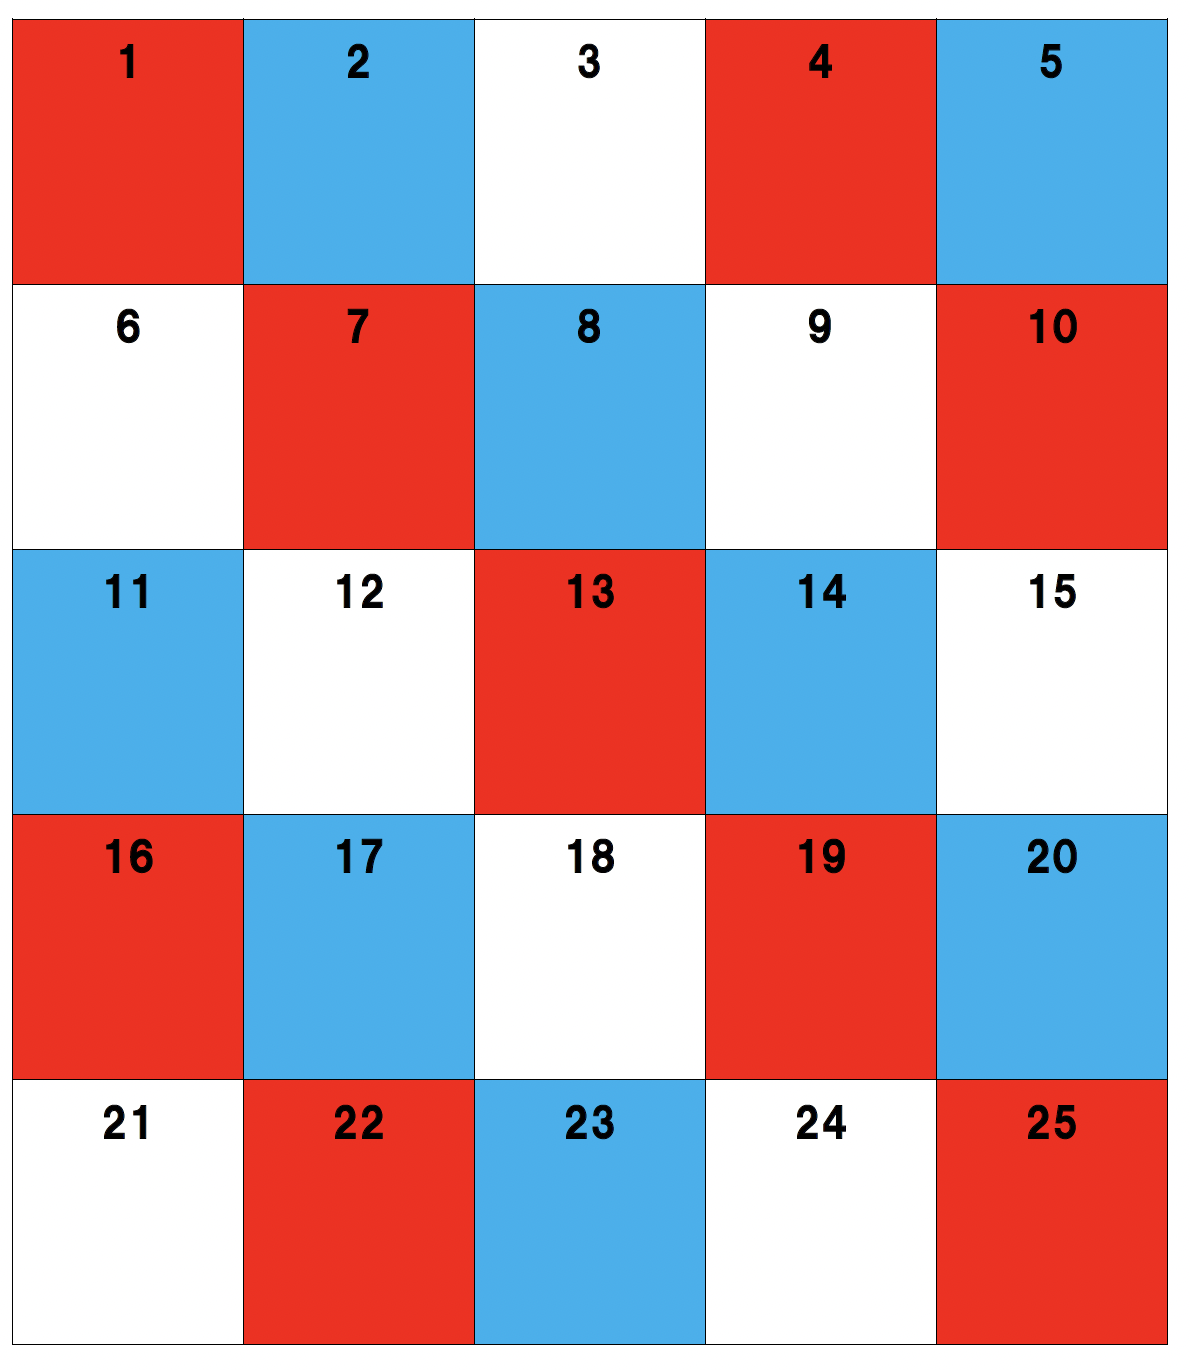
\includegraphics[width=50mm]{coin3_answer.png}
\end{center}
\end{figure}


\subsection{$1 + \sqrt{2}$}
\begin{tcolorbox}[mybox]
$(1 + \sqrt{2})^{2025}$の小数第100位を求めよ.
 \end{tcolorbox}
 
 [答え]
 $$
 (\sqrt{2} +  1)^{2025} - (\sqrt{2} - 1)^{2025}
 $$
は整数である.
 よって$ (\sqrt{2} +  1)^{2025} $はある整数から$(\sqrt{2} - 1)^{2025}$を足したものである. 
 $$
 \sqrt{2} - 1)^{2025}
 <  \left(\frac{1}{2}\right)^{2000} =  \left(\frac{1}{1024}\right)^{200} = 10^{-600}
 $$
 なので, $ (\sqrt{2} - 1)^{2025}$は小数第600位くらいに初めて0でない数字が来るかもしれない(くらい)小さい.
よって小数第100位は0である. 
 
 \begin{comment}
 \newpage
 
 \section{中田さん問題の解説}
 
問題の解答に関しては中田さんがかなり面白い解説を書いてくれたので, そこから気になったこと何個か書いていく.

\subsection{問題1}

 \begin{figure}[htbp]
\begin{center}
\includegraphics[width=50mm]{nakata1.png}
\end{center}
\end{figure}

[解説]
これ文字式を使わなくても算数的に解ける. 
$A$の$3$倍は9以下なので$A=1,2,3$のどれかである.
そして, $3$は素数なので$a$を定数として
$$
3 \cdot x \equiv a\quad \text{mod 10}
$$
となる$0 \sim 9$の数$x$はただ一つに定まる. 
よってあとは右の$3 \cdot F = A$から順番に数を定めていけば良い. 

\subsection{問題2}

 \begin{figure}[htbp]
\begin{center}
\includegraphics[width=50mm]{nakata2.png}
\end{center}
\end{figure}

これは中田さんの解答がかなり面白くてびっくりした. 
ので私がいうことはない. 

\subsection{問題3}

 \begin{figure}[htbp]
\begin{center}
\includegraphics[width=50mm]{nakata3.png}
\end{center}
\end{figure}

[解説]
これモノイドの話だと思う. 
$x_1, \ldots, x_n \in \N$について
$$
S=\{m_1x_1 + \cdots m_n x_n \mid m_i \in \N  \}
$$
とする. ある$k\in \N$があって$S \cap \{ n \in \N \mid n>k\}$の元は$x_1, \ldots, x_{n}$の最大公約数の倍数になる.(はず?)

$S$の十分大きな数に関しては$x_1, \ldots, x_{n}$の最大公約数の倍数になるということである. 今回はある十分大きな数は3と5でかけてしまうということである. 


\subsection{問題4}

 \begin{figure}[htbp]
\begin{center}
\includegraphics[width=50mm]{nakata4.png}
\end{center}
\end{figure}

これは前にも書いたし中田さんの解説もあるので省略


\subsection{問題5}

 \begin{figure}[htbp]
\begin{center}
\includegraphics[width=50mm]{nakata5.png}
\end{center}
\end{figure}

[解説]
これ天書の証明19章にもある. ちょっと見てみます...

\subsection{問題6}

 \begin{figure}[htbp]
\begin{center}
\includegraphics[width=50mm]{nakata6.png}
\end{center}
\end{figure}

[解説]
調和平均の話. これ書こうとしたら中田さんの解説にすでに書かれていた. 

\subsection{問題7}

 \begin{figure}[htbp]
\begin{center}
\includegraphics[width=50mm]{nakata7.png}
\end{center}
\end{figure}

[解説]
中田さんから問題が送られたとき, 「こんな実用的な問題が大学の問題にあったのか?」と思った.
時代ですかね.

\subsection{問題8}

 \begin{figure}[htbp]
\begin{center}
\includegraphics[width=50mm]{nakata8.png}
\end{center}
\end{figure}

[解説]
これは「格子点からなる正多角形は正方形しか存在しない」という有名事実の3角形バージョン. 
一般の場合の証明は東邦大学の土谷先生のページにある. 
\url{https://www.lab2.toho-u.ac.jp/sci/is/tsuchiya/teaching/classC/lecture/C-7.html}
みた感じピックの定理を使うっぽい

ちなみに「格子点からなる正5角形は正方形しか存在しない」という証明はもっと簡単である. 
[証明]
格子点からなる正5角形は正方形が存在したとし, 辺の長さが最小なものをとる.
今対角線を引くと, 内部にある正5角形は格子点からなる. 
(例えば右端の点から, ひだりから2番目の点の辺の長さは一番下の辺の長さに等しく, 整数なので.)
よって最小性に矛盾する.


 \begin{figure}[htbp]
\begin{center}
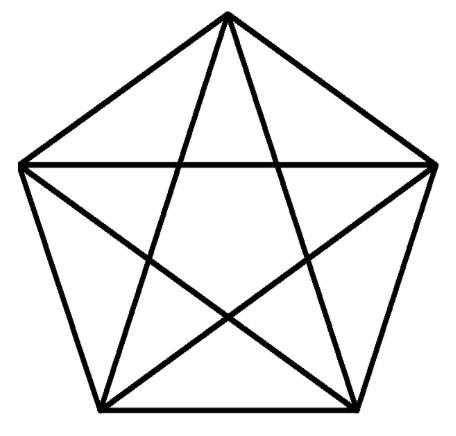
\includegraphics[width=50mm]{regular5.png}
\end{center}
\end{figure}

\subsection{問題9}

 \begin{figure}[htbp]
\begin{center}
\includegraphics[width=50mm]{nakata9.png}
\end{center}
\end{figure}

[解説] 
これも中田さんから送られた問題.
こんな図形的な問題が出てたんですね. 


\subsection{問題10}

 \begin{figure}[htbp]
\begin{center}
\includegraphics[width=50mm]{nakata10.png}
\end{center}
\end{figure}

[解説] 
いわゆるゼータ関数の問題
$$
\zeta(s):=\sum_{i=1}^{\infty}\frac{1}{n^s}
$$
とする. かの有名なオイラーは
$$
\zeta(2)=\frac{\pi^2}{6}
$$
を導き出した. 
天書の証明9章にも証明がある.
元々の証明は
$$
\frac{\sin x}{x} = \pi \prod_{n=1}^{\infty} \left( 1 - \frac{z^2}{n^2}\right)
$$
という無限乗積展開とテイラー展開を用いて示したものだと思う. 

複素解析の授業での方法は
    $$
    F(z) = \sum_{n=-\infty}^{\infty} \frac{1}{(z - n \pi)^2} \quad  G(z) =  \frac{1}{(\sin z)^2}
    $$
    とすると, $F(z), G(z)$ともに$\C$上の有理型関数で次を満たす.    
   \begin{enumerate}
   \setlength{\parskip}{0cm} 
  \setlength{\itemsep}{0cm} 
   \item $F(z + \pi)=F(z)$
   \item $z =0$の近くで$F(z) = \frac{1}{z^2} + (\text{正則関数})$
   \item $F(z)$の極は$z=n \pi$ ($n$は整数)だけである.
   \item $|Im z| \rightarrow \infty$のとき$|F(z)| \rightarrow 0$.
   \end{enumerate}
   であるので, $F(z)- G(z)$が有界正則関数になり, 定数となることから
$$
 \sum_{n=-\infty}^{\infty} \frac{1}{(z - n \pi)^2}  =  \frac{1}{(\sin z)^2}
$$
がいえる. よって
特に$z=0$の周りのテイラー展開を見ると
$$
 \sum_{n=1}^{\infty} \frac{1}{n^2}  =  \frac{\pi^2}{6}
$$
がいえるという寸法である. 
まあ頑張れば$\zeta(4)=\frac{\pi^4}{90}, \zeta(6)=\frac{\pi^6}{945}$とかも言える.

$\zeta(3)$が無理数であることはApery79による. 論文は\url{http://www.numdam.org/item/AST_1979__61__11_0/}である. 読もうとした何をやっているのかが全くわからなかった

ここまで有名な定理は簡単な証明がされていて, Wadim Zudilinの簡単な証明がある. \url{https://arxiv.org/abs/math/0202159}
これは詳細は追えないが何をやっているかはわかる. かなりelementaryな証明である. 


上の$\zeta(s)$は$\C$上の有理形関数に拡張される. 
$\zeta(-2)=\zeta(-4)=0$など負の偶数上では0になる. これを自明な零点という. 
かの有名なリーマン予想とは
\begin{tcolorbox}[mybox]
$\zeta(s)=0$なる非自明な零点は, 実部が$\frac{1}{2}$の直線上に存在する.
\end{tcolorbox}
である. まだ解けていないし解けたらクレイ数学所から100万ドルもらえる. 

\subsection{問題11}

 \begin{figure}[htbp]
\begin{center}
\includegraphics[width=50mm]{nakata11.png}
\end{center}
\end{figure}

[解説]
これかなりプログラミング的な問題である. 
プログラミングにおいて
$$
x + 5y + 10 z + 50w =1000 
$$
となる$(x,y,z,w)$を求めるとする. 
普通にfor ループを書いたら
\begin{itemize}
\item $w$を$0\sim 20$までの整数として一個とめて(for $w$ in range (0,20))
\item $z$を$0\sim 100$までの整数として一個とめて(for $z$ in range (0,100))
\item $y$を$0\sim 200$までの整数として一個とめて(for $y$ in range (0,200))
\item $x = 1000- 50w - 10z - 5y$とする. ただし$1000- 50w - 10z - 5y <0$なら無視する(if ...)
\end{itemize}
となる. 
この"$w$を一個固定していって..."の部分はプログラミングっぽい考え方である. (1)の誘導がない思いつかないと思う. 

ちなみに上のの場合$20 \times 100 \times 200=4 \times 10^5$なのでまあpythonなら2秒もかからず計算が終わる. 
多分プログラミングコンテストなら
"$x + 5y + 10 z + 50w =10^9$
となる$(x,y,z,w)$を求めるコードを求めよ. ただし処理時間2秒とする."とかで出そうである. 
(1)使えば計算量がかなり抑えられる. 

あとはかなり現実に近い問題である. 
こんな現実っぽい問題も出してたんだなあと思った. 
\end{comment}


 \end{document}
